\begin{frame}[allowframebreaks]
  \begin{figure}
    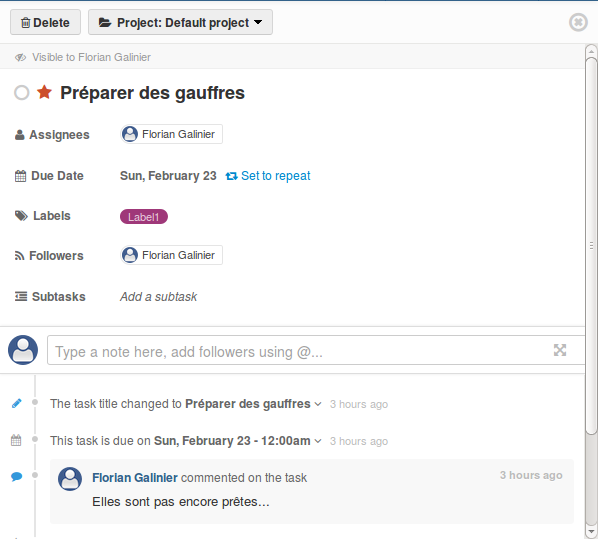
\includegraphics[scale=0.40]{img/taches.png}
  \end{figure}

\framebreak

Il est possible de : 
  \begin{itemize}
    \item modifier la priorité d'une tâche ;
    \item assigner une tâche ;
    \item définir la date limite ;
    \item créer des sous-tâches ;
    \item ajouter/retirer des labels ;
    \item laisser un commentaire sur une tâche ;
    \item définir le statut d'une tâche.
  \end{itemize}
\end{frame}